% !TEX encoding = UTF-8 Unicode

% !TEX root = ObiStein.tex

%%---------------------
%\title{Ireneo Peral y el renacer de las matem\'aticas en Espa\~na}
%\author{Yves Meyer} 
%%---------------------
%
%%---------------------
%\contact{Yves Meyer, Université Paris-Saclay}
%{yves.meyer@ens-paris-saclay.fr}{}
%%---------------------
%
%%---------------------
%\makesemititle
%%---------------------

\subsection{Ireneo Peral y el renacer de las matem\'aticas en Espa\~na}

\begin{center}\large
\textbf{Yves Meyer}\\[1em] 
\'Ecole Normale Sup\'erieure Paris-Saclay, Francia\\
{\color{azulsema}\rule{.5\linewidth}{1pt}}
\end{center}


La singular trayectoria de Ireneo Peral Alonso\footnote{No me hubiese sido posible escribir este homenaje sin la valiosa  
ayuda de Magdalena Walias, de Juan Carlos Peral y de Miguel Escobedo.} se entiende mejor si se tiene en cuenta la situaci\'on de la investigaci\'on cient{\'\i}fica en Espa\~na, a finales de los a\~nos 60, momento en el que Ireneo era estudiante. En esos a\~nos fue cuando la Escuela Matem\'atica Espa\~nola tom\'o impulso. La noche hab{\'\i}a sido profunda, larga y dolorosa. Sin embargo, algunos matem\'aticos espa\~noles de la generaci\'on anterior hab{\'\i}an procurado mantener la llama encendida. Tuve la suerte de coincidir con Ferran Sunyer i Balaguer en un congreso de an\'alisis arm\'onico en Oberwolfach en 1965, dos a\~nos antes de su muerte. Fue mucho m\'as tarde cuando conoc{\'\i} a Alberto Dou.



Espa\~na destacaba desde hac{\'\i}a tiempo por sus investigaciones en biolog{\'\i}a y medicina. La obra de Santiago Ram\'on y Cajal, completada por la de David Hubel, de Torsten Wiesel y de David Marr, conducir\'a a los trabajos revolucionarios sobre las redes de neuronas convolutivas de Yann Le Cun. El bioqu{\'\i}mico Severo Ochoa se marchar\'a de Espa\~na en 1936 para emigrar a Estados Unidos, tras una breve estancia en Alemania. Ochoa se hizo ciudadano estadounidense en 1956. Renunci\'o entonces a la ciudadan{\'\i}a  espa\~nola. Obtuvo el premio Nobel de Fisiolog{\'\i}a en 1959. Pero la Espa\~na de los estudiantes y de los investigadores seguir\'a viva en su coraz\'on. As{\'\i} es como Ochoa y Alberto Sols fundaron en 1963, mucho antes del final de la noche, la Sociedad Espa\~nola de Bioqu{\'\i}mica y Biolog{\'\i}a Molecular. En 1971 Ochoa fue nombrado director del Departamento de Biolog{\'\i}a Molecular que acababa de crearse en la nueva Universidad Aut\'onoma de Madrid. En 1975 Ochoa volvi\'o definitivamente a Espa\~na.



Pero regresemos a la matem\'aticas. En abril de 1964 Alberto Calder\'on impart{\'\i}a en la Complutense de Madrid un curso sobre An\'alisis de Fourier. Se fij\'o all{\'\i} en un estudiante especialmente brillante. Era Miguel de Guzm\'an. Calder\'on se propuso dirigir la tesis de Miguel. Miguel pas\'o entonces cuatro a\~nos en Estados Unidos, para regresar  en 1969. De vuelta a Madrid, Miguel cre\'o un grupo de investigaci\'on muy activo, y dirigi\'o numerosas tesis de doctorado, entre ellas las de Ireneo y Magdalena Walias. Algunos j\'ovenes matem\'aticos espa\~noles siguieron el ejemplo de Miguel de Guzm\'an y marcharon a Estados Unidos para empezar una tesis. Otros estudiaron en Francia. Ese fue el caso de Ildefonso D\'iaz, que defendi\'o su tesis en 1976 (directores Alberto Dou y Ha{\"\i}m Brezis), de Jes\'us Hern\'andez, que defendi\'o su tesis en 1977 (directores Ha\"im Brezis y Jos\'e Antonio Fern\'andez Vi\~na) y de Juan Luis V\'azquez que defendi\'o la suya en 1979 (directores Ildefonso D\'iaz y Ha\"im Br\'ezis). Ireneo elegi\'o quedarse en Espa\~na.



Antoni Zygmund admiraba el renacer de las matem\'aticas espa\~nolas. Pero le preocupaba que, en el campo del An\'alisis de Fourier, los j\'ovenes matem\'aticos espa\~noles se especializaran en problemas que pudieran posteriormente resultar demasiado estrechos. Yo compart{\'\i}a la misma preocupaci\'on, pero pensaba que algunos de los alumnos de Miguel de Guzm\'an ser{\'\i}an capaces de abandonar  el  puerto y  salir a navegar
en alta mar. As{\'\i} hizo Ireneo. A Ireneo le gustaban los desaf{\'\i}os arriesgados. Hacia 1980, se decant\'o por el estudio de las ecuaciones en derivadas parciales no lineales. Ten{\'\i}a 34 a\~nos y acababa de ser padre. Algunos matem\'aticos espa\~noles como  Ildefonso D\'iaz, Jes\'us Hern\'andez y Juan Luis V\'azquez hab{\'\i}an realizado su tesis en ese campo y  llevaban ya un cierto tiempo trabajando en el estudio de las ecuaciones en derivadas parciales no lineales. Cuando Ireneo decidi\'o trabajar en esa \'area   redobl\'o sus esfuerzos para alcanzar el nivel que se exig{\'\i}a a s{\'i} mismo, sin poder  beneficiarse de los consejos y \'animos de ning\'un maestro. Como escribe Cervantes, {\it cada uno es hijo de sus obras}, y esto bien puede aplicarse a Ireneo.



Las ecuaciones en derivadas parciales son uno de los m\'as bellos cap{\'\i}tulos de las matem\'aticas. Constituyen una interfaz entre las matem\'aticas y el mundo que nos rodea. Sirven para modelizar los fen\'omenos f{\'\i}sicos y predecir su evoluci\'on. Por ejemplo, las ecuaciones en derivadas parciales son esenciales en el estudio y comprensi\'on del cambio clim\'atico. Profundizar en el conocimiento de la naturaleza requiere matem\'aticas bellas y dif{\'\i}ciles. As{\'\i}, los agujeros negros y las ondas gravitacionales han sido primero soluciones de ecuaciones en derivadas parciales. No  fueron   detectados hasta mucho despu\'es, el 14 de septiembre de 2015. Pero esta eficacia tiene un precio. En primer lugar, el problema estudiado debe ser de inter\'es para la F{\'\i}sica, o la Mec\'anica (o incluso otros campos del saber). Luego, la b\'usqueda de un modelo pertinente y de herramientas matem\'aticas adecuadas es a menudo una tarea dif{\'\i}cil, que requiere una doble competencia, en Matem\'aticas y en F{\'\i}sica. Puede ocurrir que el modelo venga directamente dado  por la F{\'\i}sica y que las herramientas necesarias vengan dictadas por las leyes de conservaci\'on. Pero rara vez sucede, y m\'as a menudo el trabajo del matem\'atico consiste en descubrir lo que podr{\'\i}amos llamar nuevas leyes de conservaci\'on e incluso nuevas leyes f{\'\i}sicas. Es el caso de la simulaci\'on num\'erica de la combusti\'on en los motores de cohetes: descansa por supuesto sobre las leyes fundamentales que rigen los flujos de fluidos y las leyes de la Qu{\'\i}mica. Pero eso es todo, porque no existen todav{\'\i}a leyes propias de la combusti\'on. Finalmente, el an\'alisis matem\'atico de una ecuaci\'on en derivadas parciales es el requisito previo indispensable para su resoluci\'on num\'erica. Esta 
 requiere encontrar c\'odigos de c\'alculo eficaces. Solo entonces puede el trabajo  matem\'atico desarrollado tener aplicaciones cient{\'\i}ficas o industriales. Jacques-Louis Lions fue capaz de llevar a cabo este programa cient{\'\i}fico en su globalidad. Saludemos su influencia en el renacer de las Matem\'aticas Aplicadas espa\~nolas.
 
 
 
Tras siete a\~nos de trabajo Ireneo estaba  en condiciones de organizar, junto con Antonio C\'ordoba y Juan Luis V\'azquez, una escuela de verano sobre ecuaciones en derivadas parciales (Encuentro internacional de ecuaciones en derivadas parciales). Tuvo lugar  en la Universidad Men\'endez Pelayo de Santander del 29 de junio al 3 de julio de 1987. All{\'\i} conoci\'o Ireneo a Luis Caffarelli y Louis Nirenberg. Este \'ultimo le aconsej\'o colaborar con la Escuela Italiana. Caffarelli le 
invit\'o al Institute for Advanced Study de Princeton.


Ireneo escribi\'o 138 art{\'\i}culos. Muchos son notables, tanto por el inter\'es de los problemas estudiados como por la belleza de las herramientas matem\'aticas utilizadas. Elijo tres, de manera un tanto ego{\'\i}sta. {\it Some fourth order nonlinear elliptic problems related to epitaxial growth }  est\'a escrito en colaboraci\'on con Carlos Escudero. {\it Global existence versus blow-up results for a fourth order parabolic PDE involving the Hessian} es la continuaci\'on del anterior y es un trabajo en colaboraci\'on con Carlos Escudero y Filippo Gazzola. En estos, Ireneo y sus colaboradores estudian de manera macrosc\'opica  el crecimiento epitaxial de una capa rugosa. Es un problema que proviene de la 
f{\'\i}sica--matem\'atica y cuyas aplicaciones cient{\'\i}ficas e industriales son importantes. Las herramientas matem\'aticas utilizadas por Ireneo son absolutamente notables. Van del \textit{Mountain Pass Lemma}, en la versi\'on de Ambrosetti y de Rabinowitz, al teorema sobre la compacidad por compensaci\'on, que prolonga los resultados de Murat y Tartar y utiliza el espacio de Hardy $H^1$. Ireneo est\'a tan presente, tan vivo, en estos dos trabajos que  me gustar{\'\i}a poder hablar   todav{\'\i}a  con \'el  sobre ellos.



El tercer art{\'\i}culo del que deseo hablar es un trabajo en colaboraci\'on con Luis Caffarelli. Ireneo estaba entonces invitado (oto\~no 1992) por Caffarelli en el Institute for Advanced Study de Princeton. Utilizando de manera magistral el famoso lema de Calder\'on-Zygmund, Ireneo y Luis mejoraron las estimaciones $W^{1, p}$ para las soluciones de ecuaciones el{\'\i}pticas  en forma de divergencia. Volv{\'\i}a as{\'\i} Ireneo a las herramientas aprendidas con Miguel de Guzm\'an.


Remonto un poco en el tiempo. Invitado, el 16 de diciembre de 1981, en el seminario Goulaouic-Schwartz de la \'Ecole Polytechnique, Ireneo nos habl\'o de sus resultados recientes sobre la ecuaci\'on de ondas no lineal. Su hija mayor, Irene, ten{\'\i}a dos a\~nos y su hija peque\~na, Magdalena, uno.  
Estaba loco de felicidad por ser padre. Pero, me dec{\'\i}a, eso le  
obligaba a  mantener una disciplina estricta en la gesti\'on del tiempo.  
Deb{\'\i}a, siempre disfrutando de la presencia de sus dos hijas, intentar  
trabajar tanto como antes. En realidad estas nuevas obligaciones lo  
estimulaban. A Ireneo le gustaba enfrentarse a los desaf{\'\i}os.
Y ?`qu\'e decir de Ireneo abuelo? Su felicidad estalla en la fotograf{\'\i}a  
que acompa\~na mi testimonio. Sus cuatro nietos: Iria, \'Oscar, Laura y  
Jaime lo llenaban de orgullo.

\begin{figure}%[h]
\begin{center}
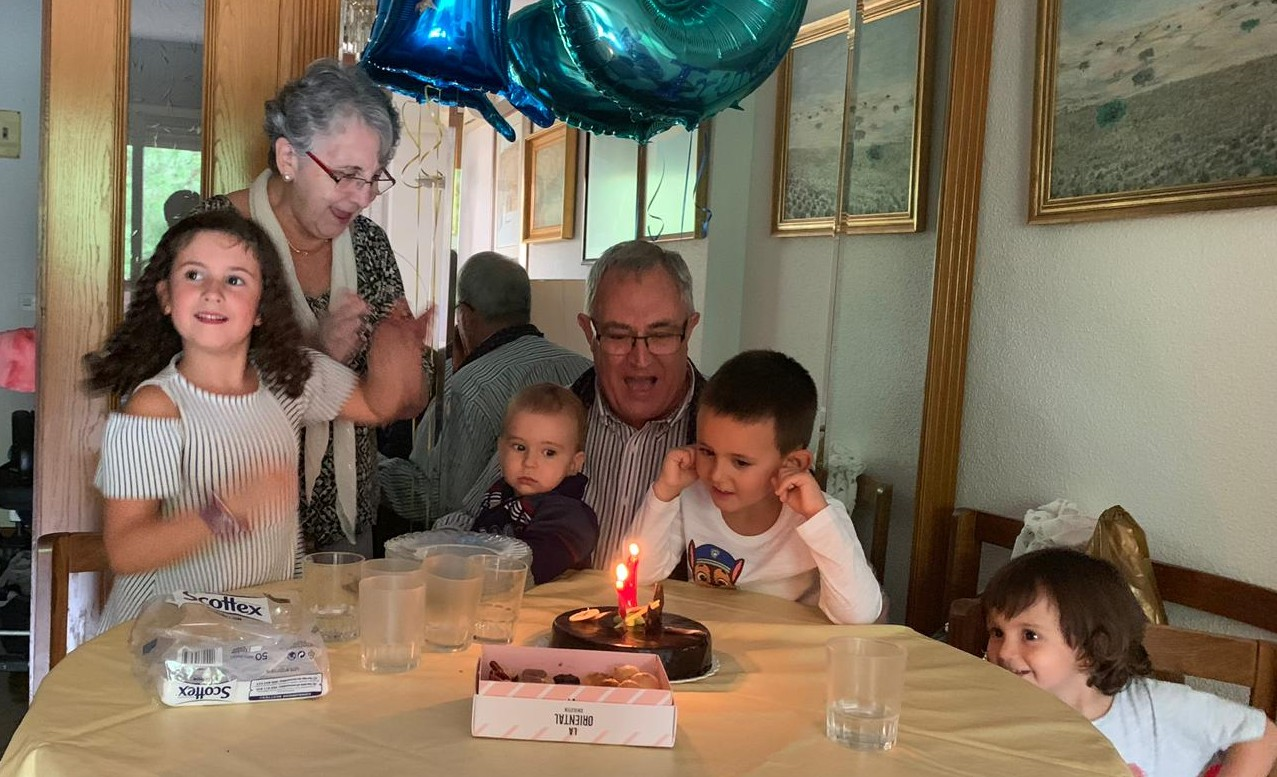
\includegraphics[width=0.9\linewidth]{IP_foto_Nietos2.jpg}
\caption{Ireneo y Magdalena con sus nietos.}
\end{center}
\end{figure}
    


Durante cuarenta a\~nos  Ireneo ha proseguido con coraje  y entusiasmo sus investigaciones sobre las ecuaciones en derivadas parciales no lineales. Amaba compartir sus ideas y entre sus colaboradores encontramos tanto los mayores nombres (como Luis Caffarelli y Antonio Ambrosetti) como los m\'as j\'ovenes y menos conocidos (como Boumediene Abdellaoui, que trabaja en Tlemcen, Argelia). Su alegr{\'\i}a de vivir y su felicidad juvenil por crear, enfrentarse y resolver problemas matem\'aticos arduos eran tan fuertes que iluminaban su vida profesional. Cuando dejaba a Ireneo, tras pasar un d\'{\i}a con \'el, recobraba \'animo, me sent{\'\i}a m\'as fuerte y el mundo era m\'as bello.
Ireneo era muy sensible y atento con  los dem\'as y, al mismo tiempo, muy exigente. La amistad y la lealtad no pod{\'\i}an desfallecer. Enseguida sent{\'\i} una gran 
simpat{\'\i}a por la pareja que Ireneo formaba con Magdalena. Frecuentarlos me llev\'o a hacerme de Espa\~na una idea diferente de la que ten{\'\i}a en mi juventud. Ireneo y Magdalena suavizaron mi visi\'on maniquea (la de la izquierda francesa). Por la fuerza y la belleza de su trabajo de investigador y por el calor de su vida familiar, Ireneo me demostraba que una Espa\~na diferente pod{\'\i}a existir, una Espa\~na que se le pareciese, realista y con talento, fuerte y generosa, liberada de los mitos del pasado. 

%
%\printcontact
%
%\endinput
%
%---------------------------


\begin{center}
\mbox{}\\[.1ex]
\resizebox{.5\linewidth}{!}{\color{azulsema}\rule{.5\linewidth}{1pt}
{\large $\diamond$} {\huge $\diamond$} {\large $\diamond$} \rule{.5\linewidth}{1pt}}
\end{center}
